\documentclass[10pt,twocolumn]{article}

\usepackage[margin=0.8in]{geometry}
\usepackage{booktabs}
\usepackage{hyperref}
\usepackage{xcolor}
\usepackage{listings}
\usepackage{microtype}
\usepackage{float}
\usepackage{tikz}
\usetikzlibrary{arrows.meta,positioning,shapes.geometric}

\raggedbottom

\lstset{
  basicstyle=\ttfamily\footnotesize,
  breaklines=true,
  frame=single,
  columns=fullflexible
}

\title{Checkpointed Exploration for DBBench Modification Tasks}
\author{Jayanth Vennamreddy}
\date{}

\begin{document}
\maketitle

\begin{abstract}
This project compares linear SQL execution with checkpointed exploration for DBBench modification tasks. In linear mode, an agent executes mutating SQL directly against a live MySQL database. In checkpointed mode, the system creates a database checkpoint before state-changing SQL, validates the result, and restores the prior state when validation fails. I also implemented a minimal autonomous SQL-agent loop that prompts an OpenAI model with the task, schema, and sample rows, then executes the generated SQL through the same checkpointing substrate. A small evaluation on DBBench dev tasks shows that checkpointing adds overhead when the first SQL action is already correct, but enables recovery when a candidate action mutates the database incorrectly.
\end{abstract}

\section{Goal}

DBBench modification tasks require an agent to issue SQL statements such as \texttt{INSERT}, \texttt{UPDATE}, and \texttt{DELETE}. Unlike read-only SQL tasks, these actions change database state. A wrong mutation can poison the session and make later reasoning unreliable. I compare a linear baseline, which executes SQL directly with no undo mechanism, against checkpointed exploration, which checkpoints the database before mutating SQL, validates the result, restores on failure, and retries an alternative action. The goal is not only to generate SQL, but to study how the execution substrate changes the failure mode of database agents.

\section{System Design}

The prototype uses a \texttt{mysql:8} Docker container as the database environment. A task loader parses DBBench JSONL records, extracts the task description, table name, columns, and initial rows, then creates a MySQL database for one task at a time. For robustness, DBBench table columns are loaded as \texttt{TEXT}; some benchmark tables contain loose scraped values that do not fit strict MySQL types such as \texttt{YEAR}.

The implementation is organized around several small components. \texttt{run\_linear.py} resets a task database and executes one SQL action directly. \texttt{run\_checkpoint.py} checkpoints the database, executes one SQL action, validates the result, and optionally restores. \texttt{run\_explore.py} tries multiple candidate SQL actions, restoring after failed validation before retrying. \texttt{run\_batch.py} runs linear and checkpointed modes on the same task set and records success, restores, and runtime. \texttt{run\_autonomous\_agent.py} builds a prompt from the DBBench task, schema, and sample rows, calls an OpenAI model to generate a candidate SQL action, and runs that action through checkpointed validation.

Each run writes both human-readable Markdown logs and structured JSON/JSONL logs. This made it possible to inspect individual failures while also producing aggregate tables. Figure~\ref{fig:architecture} summarizes the execution flow and shows where checkpointing changes the otherwise linear database-agent loop.

\begin{figure}[t]
\centering
\resizebox{\columnwidth}{!}{
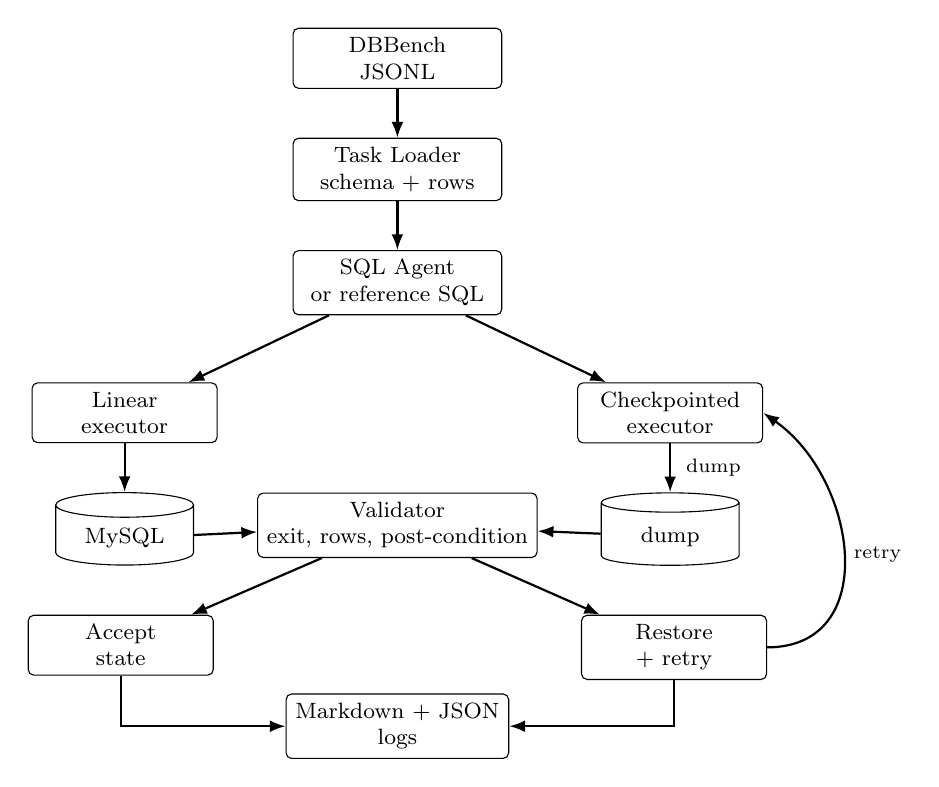
\begin{tikzpicture}[
  font=\footnotesize,
  node distance=0.62cm,
  box/.style={draw, rounded corners=2pt, align=center, minimum width=2.65cm, minimum height=0.68cm},
  smallbox/.style={draw, rounded corners=2pt, align=center, minimum width=2.35cm, minimum height=0.68cm},
  db/.style={draw, cylinder, shape border rotate=90, aspect=0.25, align=center, minimum height=0.92cm, minimum width=1.75cm},
  arrow/.style={-{Latex[length=2mm]}, thick}
]
\node[box] (jsonl) {DBBench\\JSONL};
\node[box, below=of jsonl] (loader) {Task Loader\\schema + rows};
\node[box, below=of loader] (agent) {SQL Agent\\or reference SQL};

\node[smallbox, below left=0.85cm and 0.95cm of agent] (linear) {Linear\\executor};
\node[smallbox, below right=0.85cm and 0.95cm of agent] (ckpt) {Checkpointed\\executor};
\node[db, below=0.62cm of linear] (mysql1) {MySQL};
\node[db, below=0.62cm of ckpt] (dump) {dump};

\node[box, below=2.25cm of agent] (validator) {Validator\\exit, rows, post-condition};
\node[smallbox, below left=0.72cm and 0.55cm of validator] (accept) {Accept\\state};
\node[smallbox, below right=0.72cm and 0.55cm of validator] (restore) {Restore\\+ retry};
\node[box, below=1.72cm of validator] (logs) {Markdown + JSON\\logs};

\draw[arrow] (jsonl) -- (loader);
\draw[arrow] (loader) -- (agent);
\draw[arrow] (agent) -- (linear);
\draw[arrow] (agent) -- (ckpt);
\draw[arrow] (linear) -- (mysql1);
\draw[arrow] (ckpt) -- node[right, xshift=2pt] {\scriptsize dump} (dump);
\draw[arrow] (mysql1) -- (validator);
\draw[arrow] (dump) -- (validator);
\draw[arrow] (validator) -- (accept);
\draw[arrow] (validator) -- (restore);
\draw[arrow] (restore.east) to[out=0,in=-35,looseness=1.25] node[right] {\scriptsize retry} (ckpt.east);
\draw[arrow] (accept) |- (logs);
\draw[arrow] (restore) |- (logs);
\end{tikzpicture}
}
\caption{Prototype architecture. The same DBBench task and candidate SQL action can be executed through either the linear baseline or the checkpointed exploration path.}
\label{fig:architecture}
\end{figure}

\section{Checkpointing and Validation}

Before state-changing SQL, checkpointed mode creates a dump:

\noindent\fbox{%
\begin{minipage}{0.95\columnwidth}
\ttfamily\footnotesize
mysqldump -uroot -prootpass dbbench \textgreater{} /tmp/dbbench\_checkpoint.sql
\end{minipage}}

If validation fails, it restores the database:

\noindent\fbox{%
\begin{minipage}{0.95\columnwidth}
\ttfamily\footnotesize
mysql -uroot -prootpass dbbench \textless{} /tmp/dbbench\_checkpoint.sql
\end{minipage}}

The current validator checks whether the SQL command returned a successful exit code, whether the number of affected rows matched an expected value, whether the table row-count delta matched the task type, and whether a post-condition query returned the expected row. For simple \texttt{INSERT ... VALUES ...} reference statements, the system can infer this post-condition automatically by converting the inserted table, columns, and values into an exact-row \texttt{SELECT} query.

For example, for the Madison High School insertion task, the post-condition was:

\begin{lstlisting}[language=SQL]
SELECT * FROM `School Location Table`
WHERE `School` = 'Madison High School'
  AND `Location` = 'San Diego';
\end{lstlisting}

\section{Results}

Table~\ref{tab:batch} shows a five-task DBBench dev run using reference SQL actions. In this controlled setting, both modes succeed because the SQL is already correct. Checkpointed mode adds dump overhead, but creates a restore boundary before mutation.

\begin{table}[H]
\centering
\scriptsize
\setlength{\tabcolsep}{2.8pt}
\begin{tabular}{lcccrr}
\toprule
Task & Type & Lin. & Ckpt. & Lin. (s) & Ckpt. (s) \\
\midrule
m0 & INSERT & pass & pass & 0.0858 & 0.1693 \\
m1 & INSERT & pass & pass & 0.0767 & 0.2162 \\
m2 & INSERT & pass & pass & 0.0773 & 0.1616 \\
m3 & INSERT & pass & pass & 0.0716 & 0.1637 \\
m4 & INSERT & pass & pass & 0.0656 & 0.1477 \\
\bottomrule
\end{tabular}
\caption{Linear vs checkpointed execution on five DBBench dev modification tasks using reference SQL. Checkpointed runs created one checkpoint and performed zero restores in this controlled batch.}
\label{tab:batch}
\end{table}

In addition to the controlled reference-SQL runs, I tested the autonomous SQL-agent path on the Madison High School insertion task. The model generated the correct \texttt{INSERT} statement on the first attempt; checkpointed validation accepted the mutation, and no restore was needed. This verifies that the prompt-generation and model-action loop can plug into the same execution and validation substrate used by the controlled experiments.

\section{Case Analysis}

\textbf{Checkpointing helped.} In one exploration run, the first candidate inserted \texttt{Wrong High School}. The SQL executed successfully and affected one row, so a simple SQL-error check would not catch the mistake. However, the post-condition query for \texttt{Madison High School} returned no rows. The system restored the checkpoint and tried the second candidate, which inserted the correct row and passed validation.

\textbf{Checkpointing did not help.} In another run, both candidate SQL actions inserted semantically wrong rows. Checkpointing restored the database after each failed attempt, but no candidate satisfied the task. This shows that checkpointing protects state but does not by itself solve misunderstanding of the task or schema.

\textbf{Overhead was not worth it.} In the reference-SQL batch, the first SQL action was already correct for every task. Checkpointing still succeeded, but added roughly 0.08--0.14 seconds per task from dump overhead. This suggests checkpointing is most useful when actions are uncertain or potentially destructive.

\section{Limitations and Next Steps}

This prototype uses DBBench reference SQL for the initial batch, so that experiment primarily measures checkpoint overhead rather than full LLM-agent performance. I added a minimal autonomous OpenAI SQL generator and tested it on one task, but a broader evaluation of generated SQL across the full dev set remains future work. The retry experiments still simulate some bad candidate SQL manually in order to isolate the restore-and-retry behavior.

Future improvements include using transaction savepoints when possible instead of full \texttt{mysqldump}, restoring by replaying accepted action prefixes, building stronger schema-aware validators, adding safer SQL generation that selects target rows before mutating, and evaluating all DBBench dev modification tasks.

\section{Conclusion}

The experiment shows that checkpointed exploration changes the failure model for database agents. Linear execution is fast but brittle: once a wrong mutation is applied, the session is corrupted. Checkpointing adds overhead, but creates a recoverable boundary that allows an agent to inspect, reject, restore, and retry. The main research challenge is not only checkpoint creation, but deciding when a mutation should be accepted.

\end{document}
